\chapter{Implementation von Beispielapps}
\label{implementation}
\section{Allgemein}
\subsection{Spiellogik}
\subsubsection{Server}
Der implementierte Server arbeitet mit Java und ZeroMQ. Er �ffnet zwei Kommunikationskan�le mit dem Client. Der erste ist ein ZeroMQ-Request-Reply-Socket-Paar, �ber das die Endger�te Nachrichten an den Server senden. Der zweite ist ein Publish-Subscribe-Socket-Paar, �ber das die Nachrichten an Gruppen von Endger�ten weitergeleitet werden. Eine Nachricht besteht aus drei Teilen: einer Adresse, dem Nachrichtentyp und einem serialisierten Objekt vom Typ TransferObject (siehe Abbildung \ref{fig:transfer}). Die Adresse ist entweder die ID eines Spielers oder die ID einer Spielinstanz. Wir nutzen ZeroMQs Multipart-Message-Feature um diese Teile voneinander getrennt bei der Kommunikation zu �bermitteln. Der Server sendet eingehende Nachrichten an bestimmte Clients weiter. Das kann entweder ein einzelner Client, oder alle Clients die sich in einer Spielsession befinden, sein. Der Server kennt dabei den Zustand der einzelnen Spiele nicht. , Um mehrere Spielinstanzen gleichzeitig verwalten zu k�nnen, h�lt er aber eine Liste aller laufenden Spiele samt Informationen dar�ber, welcher Spieler an welchem Spiel teilnimmt. Wenn eine Nachricht vom Typ \glqq create\_game\grqq empfangen wird tr�gt der Server die ID des Spiels in eine Liste ein. Diese Liste wird einem Client gesendet wenn er sie �ber eine entsprechende Nachricht anfragt.



\begin{figure}
	\begin{center}
		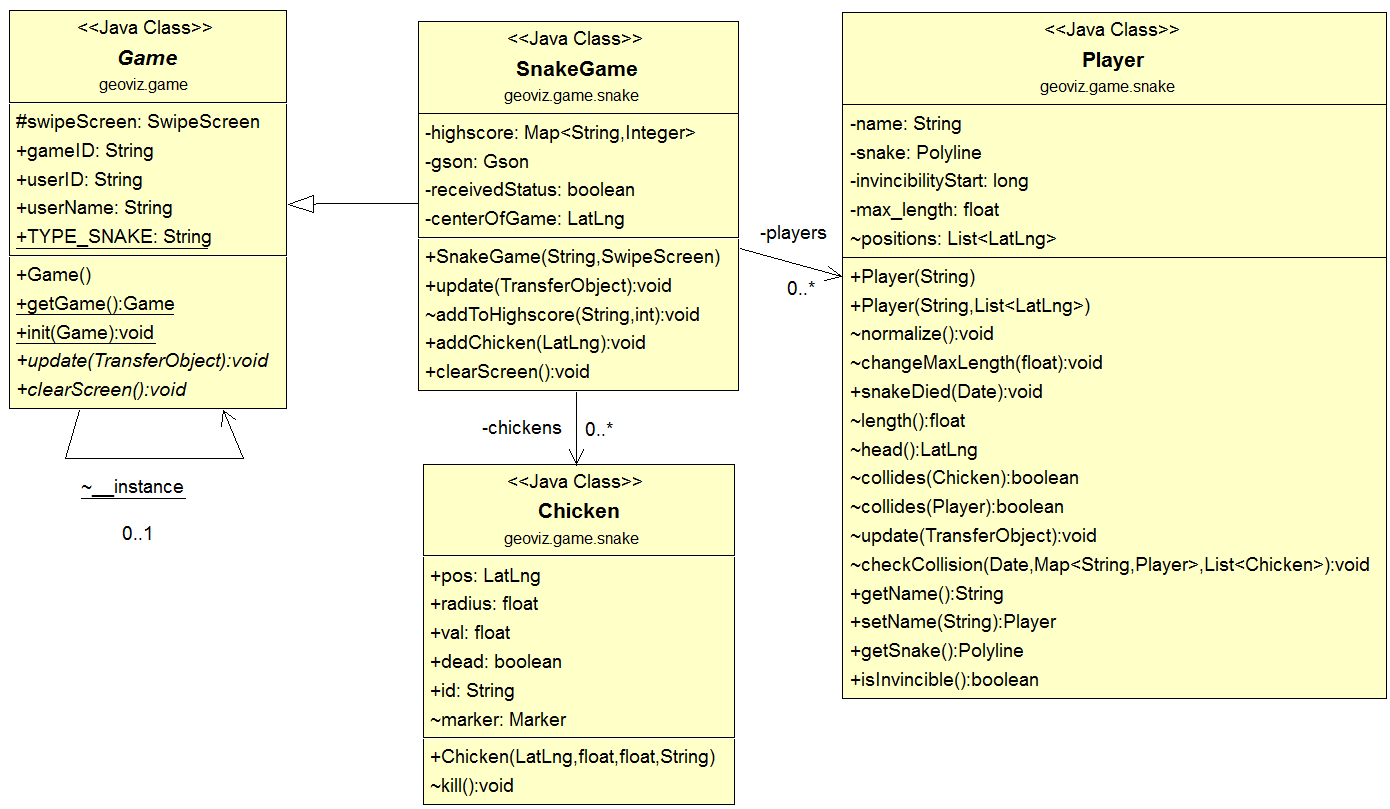
\includegraphics[width=1\textwidth]{img/snake.png}
	\end{center}
	
	\caption{UML-Diagramm zur Spiellogik}
	\label{fig:snake}
\end{figure}

\subsubsection{Client}
Unsere Android-Applikation besteht aus drei Fragmenten zwischen denen man durch Wischen wechseln kann. Das erste Fragment ist ein Chat über den Spieler Textnachrichten an ihre Mitspieler im gleichen Spiel senden können.
Das zweite Fragment ist die Karte auf der wir unser Spiel darstellen.  
Für die Darstellung der Karte verwenden wir GoogleMaps. 
Im dritten Fragment kann ein Spieler eine neue Spielinstanz erstellen oder einem bereits laufendem Spiel beitreten. Die Liste der momentan laufenden Spiele wird per Knopfdruck vom Server abgefragt. Wenn man einer laufenden Session beitritt wird über den Server eine Anfrage des aktuellen Status des Spiels an alle momentanen Mitspieler gesendet, welche den Zustand des Spiels alle an den anfragenden Client zurück senden. Dieser beachtet nur die erste Nachricht und verwirft den Rest.
Des weiteren läuft ein LocationClient, welcher immer die aktuelle Position als Nachricht an alle Spieler der selben Spielinstanz weiterschickt. 

\section{Der Android Client}

\subsection{Aufbau der GUI}

GUIIIIIIIIIIIIIIIIIIIIIIIIIIIIIIIIIIIIIIIIIIIIIIIIIIIIIIIIIIIIIIIIIIIIIIIIIIIIIIIIIIIIIIIIIIIIIIII
IIIIIIIIIIIIIIIIIIIIIIIIIIIIIIIIIIIIIIIIIIIIIIIIIIIIIIIIIIIIIIIIIIIIIIIIIIIIIIIIIIIIIIIIIIIIIIIIII
IIIIIIIIIIIIIIIIIIIIIIIIIIIIIIIIIIIIIIIIIIIIIIIIIIIIIIIIIIIIIIIIIIIIIIIIIIIIIIIIIIIIIIIIIIIIIIIIII

\subsection{Kommunikation}

blablablablablablablablablab lablablablabla blablablabla blablablablablablab  lablablablab lablablablab labla
blablablablablab lablablablablablablabla blablablablablablablablablablablablab lablablablablabl ablablabla
blablablablablablablablablablablablablablablablablablablablablablablablablablablablablablablablablabla
blablablab lablablablabla blablablablablablablabl  ablablablablablablablablabl ablabla blablablablablablabla
blablablablablablablablablablablablablablablablablablablablablablablablab lablablablablablablablablabla
blablablablablablabla blablablablablablablablablablablablablablablablablablablablablablablablablablabla
blablablablablablablablablablablablablablablablablablablab lablablablablablablablablabla  blablablablabla
blablablablablablablablablablablablablablablablablablablablablablablablablablablablablablablablablabla
blablablablab lablablablablablabl ablablablablablablablablablablablablablablablablablablablablablablabla
blablablablablablablablablablablablablablablablablablab ablablablablablablabl ablablablablablablablabla
\subsection{Die Karte}

\subsubsection{OpenStreetMap vs. GoogleMaps}

READY????! 3 2 1 FIGHT!!!!!!!!!!!!!!
\subsubsection{Fazit}

AAAAAAND the WINNNNNNER ISSSSS ..........
\subsection{Die Karte}

\subsubsection{LocationManager vs. LocationClient}

READY????! 3 2 1 FIGHT!!!!!!!!!!!!!!
\subsubsection{Fazit}

AAAAAAND the WINNNNNNER ISSSSS ..........
\subsection{Spiellogik}

Lebe lange und in Frieden.

\section{Snake}


\subsection*{Spielidee}
Das zweite Spiel, das von uns umgesetzt wurde, ist ein Flaggenspiel. Hierbei handelt es sich um eine Abwandlung von Capture the Flag. Es wird mit Stealth-Elementen erweitert und die Spielmechanik des Ausschaltens von Gegnern ist anders gel�st. Dieses Spiel sollte nach M�glichkeit in einer Stadt gespielt werden, da es wichtig ist in einer Menge von Passanten m�glichst unerkannt zu bleiben. Es gibt zwei Teams, die jeweils eine Basis haben. Basen werden jeweils von dem Mitglied eines Teams erstellt, welches als erstes die Erstellung �ber einen Button ausl�st. Hierbei wird als Zentrum der Basis die aktuelle Position des entsprechenden Spielers genommen. Beim betreten des Spiels, k�nnen sich Spieler zwischen Team Blau und Team Rot entscheiden. Die eigene Flagge erscheint in der N�he der eigenen Basis. Die Position der eigenen Flagge ist den Teammitgliedern unbekannt, man sieht nur die Position der gegnerischen Flagge. Die Flaggen sollen nur auf Stra�en bzw. Gehwegen (nicht in Geb�uden) zuf�llig platziert werden. Diese Platzierung wird vom Server �ber Bilderkennung bestimmt. So wird die Erreichbarkeit der Flaggen sichergestellt. Als Spieler sieht man nur die Positionen der eigenen Teammitglieder. Zur Organisation kann der Chat verwendet werden. Es ist m�glich die n�here Umgebung nach Gegnern zu scannen. Die gescannten Gegner sind dann f�r kurze zeit sichtbar. Dieses Scan-Verfahren ist jedoch nicht dauerhaft verf�gbar, sondern erst wieder m�glich nach l�ngerer Abklingzeit. Es ist m�glich potentielle Gegner zu markieren. Die Reichweite beim Markieren ist begrenzt und Richtungsabh�ngig. Hierbei wird das Smartphone auf den potentiellen Feind ausgerichtet und ein Mark-Button gedr�ckt (Auch hier besteht eine gewisse Abklingzeit). Ist dieser ein gegnerischer Mitspieler wird er markiert und ist f�r l�ngere Zeit auf der Karte sichtbar. Der Betroffene bekommt �ber seine Markierung keine R�ckmeldung. Ein Spieler, der sich in der N�he der gegnerischen Flagge befindet, kann diese aufnehmen. Um einen Spiel-Punkt zu erreichen muss die aufgenommene Flagge zur eigenen Basis gebracht werden. Dem Gegnerteam wird die Position angezeigt, an der die Flagge aufgenommen wurde. Wird ein Flaggentr�ger markiert, verliert er die Flagge und sie erscheint an einer neuen zuf�lligen Position. War der Flaggentr�ger vor der Aufnahme markiert, so ist er mit Flagge zu sehen. Wenn ein Spieler eine bestimmte Geschwindigkeit �berschreitet, wird er ebenfalls f�r das Gegnerteam sichtbar. Somit haben schnellere L�ufer keinen direkten Vorteil.
\begin{figure}
	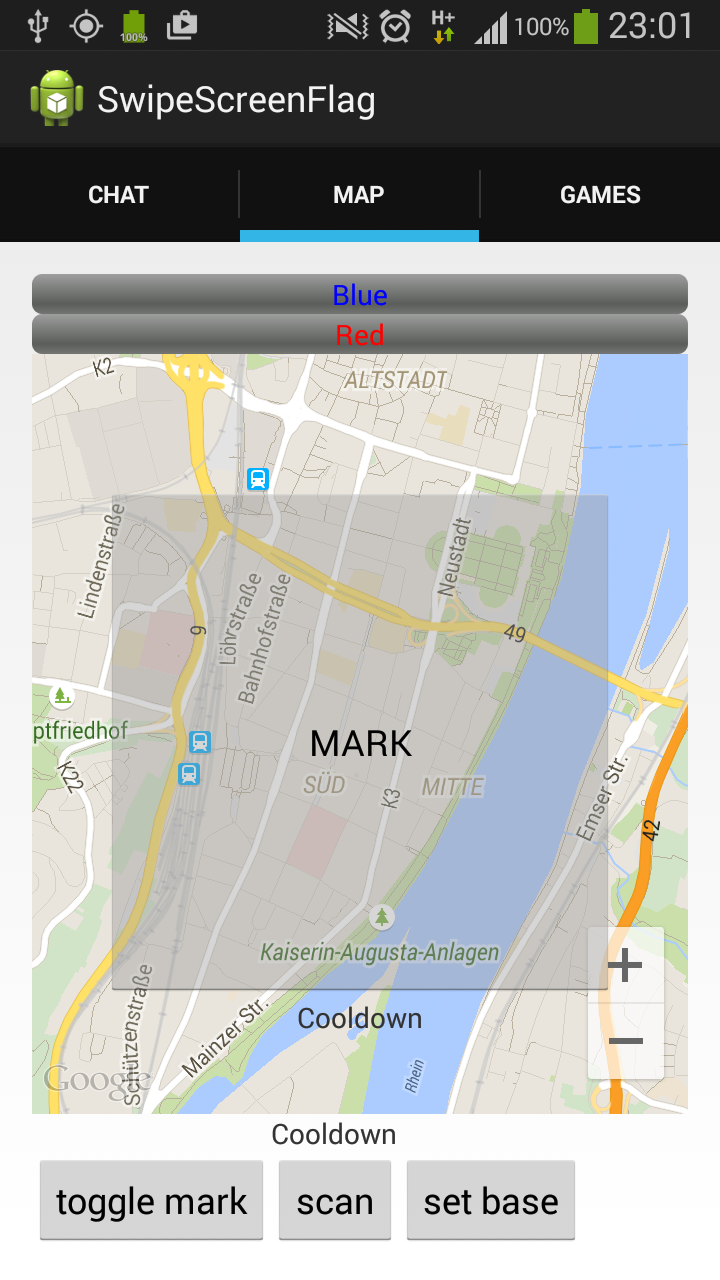
\includegraphics[width=0.5\textwidth]{5-Implementation_von_Beispielapps/5-2-Verstecken/Data/map_screen_mark_on.png}
	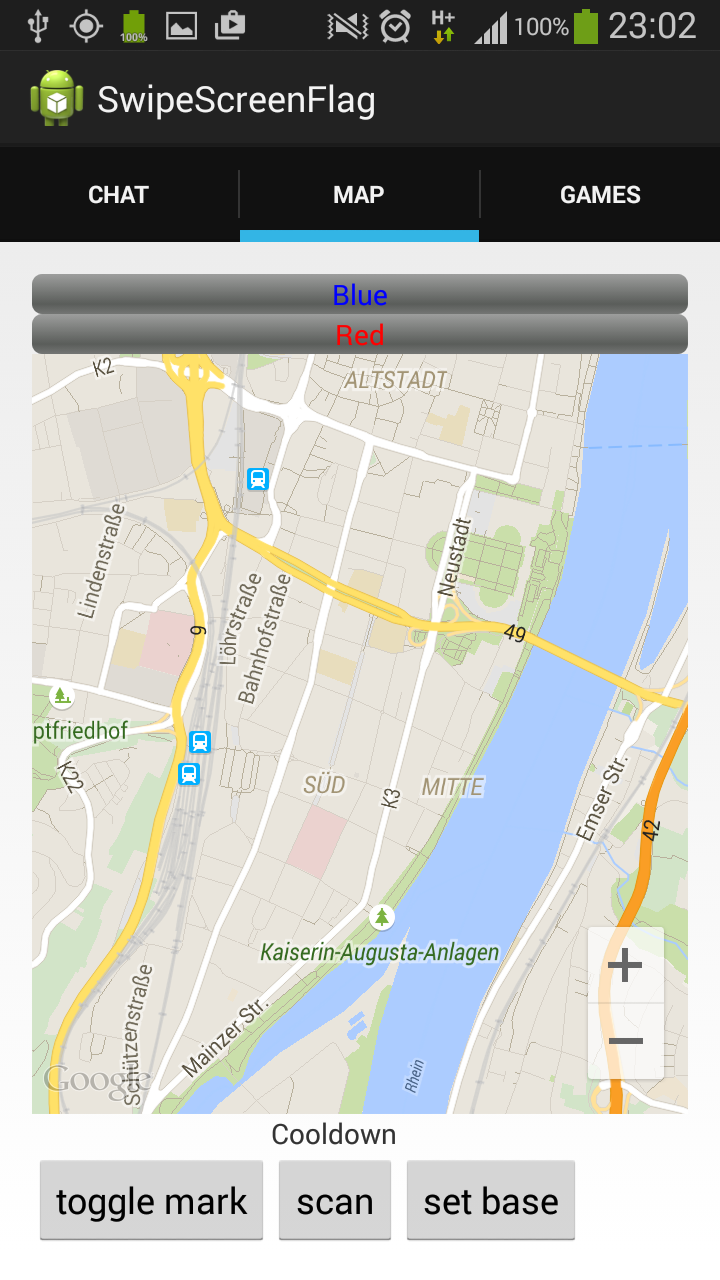
\includegraphics[width=0.5\textwidth]{5-Implementation_von_Beispielapps/5-2-Verstecken/Data/map_screen_mark_off.png}
	\caption{Map-Screen mit Mark-Button (rechts) Map-Screen ohne Mark-Button (Links)}
	\label{fig:flaggmap}
\end{figure}


\subsection{Spiellogik}

\subsubsection*{Server}
Der Server wird hier noch mit einer Zusatzfunktion ausgestattet. Er generiert nach vorher festgelegten Bedingung g�ltige Flaggenpunkte. In diesem Fall z�hlen Stra�en als g�ltige Punkte. Der Server ruft �ber GoogleStaticMap einen Kartenabschnitt ab, auf dem der Flaggenpunkt generiert werden soll. Nun wird ein zuf�lliger Pixel in der Mitte des Bildes nach der Farbe �berpr�ft. Stimmt dieser mit der Farbe von Stra�en �berein, wird diese Position als g�ltig zur�ck �bertragen und der Flaggenpunkt kann generiert werden. Ist die Farbe ung�ltig wird ein entsprechender neuer Kartenabschnitt aufgerufen und die Prozedur beginnt erneut.

\subsubsection*{Client}
Auf der Client-Seite wird die Sichtbarkeit der Spieler und Objekte (Flaggen und Basen) gehandhabt.

\paragraph{Markieren}
 S�mtliche Positionen sind den Gerten bekannt, aber nicht alle sichtbar. Damit verbunden sind auch die Funktionalit�ten des Markieren und Scannens. F�r das Markieren werden jeweils die beiden Koordinaten des Markierenden (A) und des Markierten (B), sowie den Sichtkegel von A und eine Reichweite ben�tigt. 
F?r den Sichtkegel ben�tigt man einen Orientierungswinkel ($\alpha$), welche mittels der Sensoren f�r Orientierung (s. \ref{orientierung}) ermittelt wird, sowie einen vorher festgelegten Winkel f�r den Sichtbereich ($\beta$). Nun wird der Winkel der beiden Punkte A und B ($\gamma$) bestimmt (s. \ref{abstandsmessung}).


Liegt $\gamma$ im Intervall $[ \alpha - \frac{\beta}{2}; \alpha + \frac{\beta}{2}]$ und ist die Distanz zwischen A und B innerhalb der Reichweite, so gilt B als markiert. �ber eine Nachricht wird den anderen Teammitgliedern mitgeteilt das B jetzt markiert und somit f�r eine gewisse Zeit sichtbar ist. A kann f�r eine vordefinierte Zeit keine weiteren Gegner markieren.

\paragraph{Scannen}

Um einen festgelegten Radius eines Spielers nach Gegnern zu scannen, wird die Distanz (s. \ref{abstandsmessung}) zwischen dem Scannenden (C) und allen gegnerischen Spielern ermittelt. C werden, f�r eine kurze Zeit, alle gegnerischen Spieler angezeigt, die sich innerhalb eines bestimmten Distanzwertes befinden. Die M�glichkeit zu Scannen steht C f�r eine gewisse Zeit nicht mehr zur Verf�gung.

\paragraph{Geschwindigkeits�berpr�fung}
Es existiert eine st�ndig aktive Geschwindigkeits�berpr�fung der Spieler durch ihre Koordinaten (s. \ref{locationManager}). Wenn eine feste Maximalgeschwindigkeit durch einen Spieler �berschritten wird, schickt der entsprechende Client eine Nachricht an alle gegnerischen Ger�te, dass dieser angezeigt werden soll. Wird die Maximalgeschwindigkeit wieder unterschritten, ist der Betroffene wieder unsichtbar f�r die Gegner

\paragraph{Basen- und Flaggenplatzierung}
Die Basis eines Teams wird vom ersten Teammitglied gesetzt, welches auf den "`set Base"' Button klickt. Als Zentrum wird die momentane Position des Spielers genommen. Die Darstellung erfolgt als Kreis. Nun wird in einem vorher festgelegtem Radius um die Basis zuf�llig die Teamflagge platziert. Die Auswahl f�r eine g�ltige Koordinate trifft dabei der Server und teilt dies den entsprechenden Mitspielern �ber eine Nachricht mit. Die aktuelle Position der Flagge wird jedoch dem eigenen Team nicht angezeigt. Wird die Flagge von einem Mitspieler des gegnerischen Team gestohlen, werden die betroffenen Spieler �ber einen Vibrationsalarm informiert. Auch wird die letzte Position der Flagge vorl�ufig angezeigt. Wenn der Flaggentr�ger gestoppt wird, generiert der Server wieder eine g�ltige Position f�r eine neue Flagge 
\subsection*{Umgesetzte Features}
%aaaaaaaaarg gkls akj dasdlj ad ka kd askd 
Zus�tzlich zu den im Zuge der Implementation von Snake umgesetzten Features wurde die Geschwindigkeitsmessung (siehe Abschnitt \ref{sec:geschwindigkeitsmessung}) implementiert. F�r das Markieren wurde au�erdem eine Richtungsangabe (siehe Abschnitt \ref{sec:richtungsangabe}) ben�tigt.

